% Options for packages loaded elsewhere
\PassOptionsToPackage{unicode}{hyperref}
\PassOptionsToPackage{hyphens}{url}
%
\documentclass[
]{article}
\usepackage{lmodern}
\usepackage{amssymb,amsmath}
\usepackage{ifxetex,ifluatex}
\ifnum 0\ifxetex 1\fi\ifluatex 1\fi=0 % if pdftex
  \usepackage[T1]{fontenc}
  \usepackage[utf8]{inputenc}
  \usepackage{textcomp} % provide euro and other symbols
\else % if luatex or xetex
  \usepackage{unicode-math}
  \defaultfontfeatures{Scale=MatchLowercase}
  \defaultfontfeatures[\rmfamily]{Ligatures=TeX,Scale=1}
\fi
% Use upquote if available, for straight quotes in verbatim environments
\IfFileExists{upquote.sty}{\usepackage{upquote}}{}
\IfFileExists{microtype.sty}{% use microtype if available
  \usepackage[]{microtype}
  \UseMicrotypeSet[protrusion]{basicmath} % disable protrusion for tt fonts
}{}
\makeatletter
\@ifundefined{KOMAClassName}{% if non-KOMA class
  \IfFileExists{parskip.sty}{%
    \usepackage{parskip}
  }{% else
    \setlength{\parindent}{0pt}
    \setlength{\parskip}{6pt plus 2pt minus 1pt}}
}{% if KOMA class
  \KOMAoptions{parskip=half}}
\makeatother
\usepackage{xcolor}
\IfFileExists{xurl.sty}{\usepackage{xurl}}{} % add URL line breaks if available
\IfFileExists{bookmark.sty}{\usepackage{bookmark}}{\usepackage{hyperref}}
\hypersetup{
  pdftitle={Benefit Threat to City Solvency},
  pdfauthor={Questions: citysolvency@ncf.edu},
  hidelinks,
  pdfcreator={LaTeX via pandoc}}
\urlstyle{same} % disable monospaced font for URLs
\usepackage[margin=1in]{geometry}
\usepackage{graphicx}
\makeatletter
\def\maxwidth{\ifdim\Gin@nat@width>\linewidth\linewidth\else\Gin@nat@width\fi}
\def\maxheight{\ifdim\Gin@nat@height>\textheight\textheight\else\Gin@nat@height\fi}
\makeatother
% Scale images if necessary, so that they will not overflow the page
% margins by default, and it is still possible to overwrite the defaults
% using explicit options in \includegraphics[width, height, ...]{}
\setkeys{Gin}{width=\maxwidth,height=\maxheight,keepaspectratio}
% Set default figure placement to htbp
\makeatletter
\def\fps@figure{htbp}
\makeatother
\setlength{\emergencystretch}{3em} % prevent overfull lines
\providecommand{\tightlist}{%
  \setlength{\itemsep}{0pt}\setlength{\parskip}{0pt}}
\setcounter{secnumdepth}{-\maxdimen} % remove section numbering
\usepackage{booktabs}
\usepackage{longtable}
\usepackage{array}
\usepackage{multirow}
\usepackage{wrapfig}
\usepackage{float}
\usepackage{colortbl}
\usepackage{pdflscape}
\usepackage{tabu}
\usepackage{threeparttable}
\usepackage{threeparttablex}
\usepackage[normalem]{ulem}
\usepackage{makecell}
\usepackage{xcolor}

\title{Benefit Threat to City Solvency}
\author{Questions:
\href{mailto:citysolvency@ncf.edu}{\nolinkurl{citysolvency@ncf.edu}}}
\date{5/1/2020}

\begin{document}
\maketitle

\hypertarget{executive-summary}{%
\section{Executive Summary}\label{executive-summary}}

The unfunded obligations of the pension and other post-employment
benefits (OPEB) plans sponsored by local governments in the United
States continue to grow. In the following report, we study in detail the
financial obligations of 21 of the 22 largest US cities (excluding
Washington, DC, the 20th largest city). We review both their own reports
on these obligations and how these differ from our estimates based on
more realistic assumptions.

We find that most cities reported OPEB liabilities close to our
measures, however, for pensions, we find that cities drastically
undervalue their unfunded liabilities. In fact, at the end of the 2017
fiscal year, these largest U.S cities reported unfunded liabilities of
approximately \textbf{\$545} billion: \textbf{\$432} billion for
pensions and \textbf{\$113} billion for OPEB. According to our
calculations, we estimate the true unfunded liabilities to be over
\textbf{\$803} billion: \textbf{\$672} trillion for pensions and
\textbf{\$131} billion for OPEB.

The largest discrepancy, between the unfunded pension liabilities
reported by the cities and our estimates of their pension liabilities,
is primarily the result of different discount rates used in valuing
these liabilities. Under government accounting standards, cities are
given broad discretion to choose a discount rate based on their
expectation of future returns on plan assets. Thus, there is wide
variation in the discount rate chosen by cities in their reporting, with
several cities choosing highly optimistic discount rates for their
pension plans at 7\% or higher (see appendix).

But discount rates are supposed to represent a conservative rate of
return with a high degree of confidence. For example, the FASB
stipulates that corporations must use the AA corporate bond rate as the
discount rate for their pension plans. In June, 2017, the AA corporate
bond rate for 15 years was approximately 4\%. Therefore, we used that
4\% as the discount rate in our estimates of the unfunded liabilities
for pensions in all 21 cities, and a 3\% discount rate for OPEBs to
account for the comparably shorter liabilities of OPEBs relative to
pensions.

Our analysis is divided into three main parts. First, we present in
detail the unfunded pension liability of the 21 cities, followed by
pension liability per capita and pension liability as a percentage of
revenues. Second, we present in detail the unfunded OPEB liability of
the 21 cities, followed by OPEB liability per capital and OPEB liability
as a percentage of revenues. Third, we present total pension and OPEB
liabilities for each city, followed by total liabilities per capita and
as share of revenue.

\hypertarget{i.-pension-liability}{%
\section{I. Pension Liability}\label{i.-pension-liability}}

In this section, we study in detail the pension liability of the 20
cities. We report on both the city's own calculations of their pension
obligations, based on their Comprehensive Annual Financial Reports
(CAFRs), and illustrate how these differ from valuations using a
standardized discount rate calculation. First, we present the total
unfunded pension liability for each city in dollars. Second, we showcase
the total liability scaled by population size. Finally, we present the
2017 pension expense as a share of governmental fund revenues.

\hypertarget{total-pension-liability}{%
\subsubsection{1. Total Pension
Liability}\label{total-pension-liability}}

The difference in the reported pension liability and the ones calculated
under our standardized valuation are illustrated in Figure 1 below. In
general, the higher discount rates used by cities in their calculations
result in much lower - sometimes, dramatically lower - estimates of
their unfunded liabilities, with cities like New York, Los Angeles, and
Chicago reporting particularly extreme total differences. Even cities
without extreme values generally report a value notably lower than the
standardized value, with only Fort Worth reporting an unfunded pension
liability close to our standardized measure.

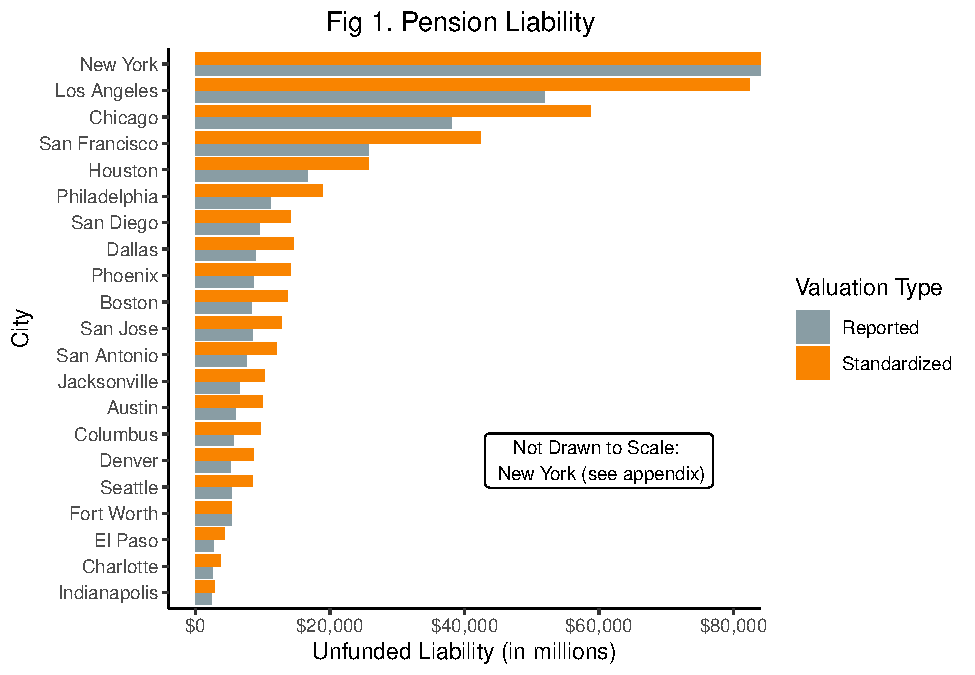
\includegraphics{City-Solvency-Report--Adjusted-_files/figure-latex/unnamed-chunk-6-1.pdf}

\hypertarget{total-pension-liability-per-capita}{%
\subsubsection{2. Total Pension Liability Per
Capita}\label{total-pension-liability-per-capita}}

To better illustrate the scale of concern for unfunded pension
liability, we provide per capita measures to represent a city's pension
financial burden relative to their population size. This also allows
comparisons with other cities more naturally. As before, city
obligations are under-reported in reported values, with the average
reported total pension liability per capita was \textbf{\$8,934} while
the average standardized total pension liability per capita was
\textbf{\$14,035}.

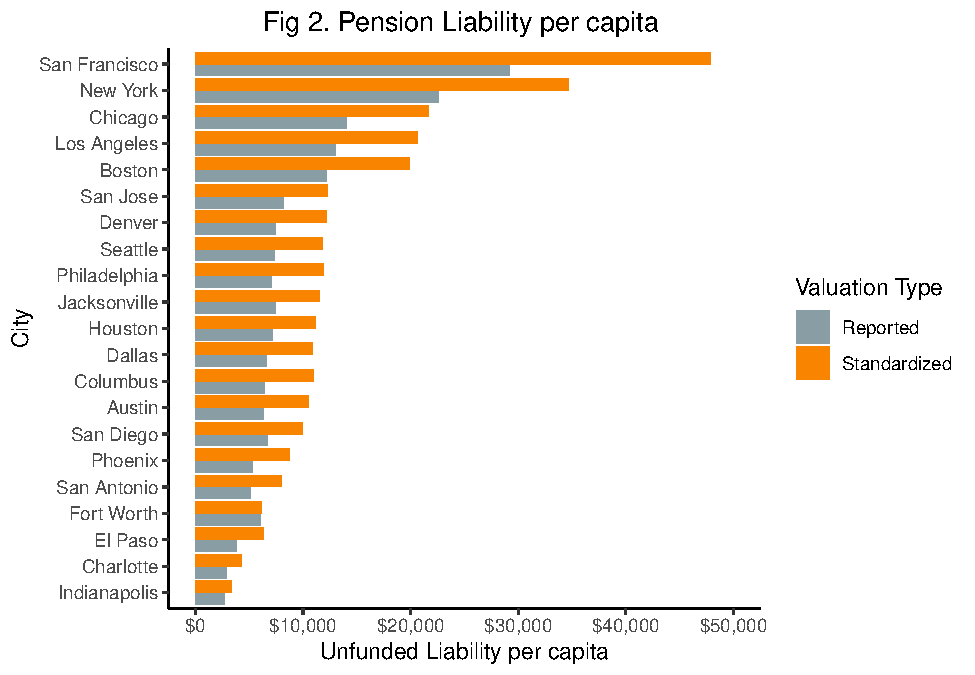
\includegraphics{City-Solvency-Report--Adjusted-_files/figure-latex/unnamed-chunk-7-1.pdf}

Furthermore, the variation in city obligation becomes clearer, as some
cities appear to be in more extreme fiscal danger while others appear to
have more manageable situations, relative to their populations (and
thus, potential tax base). As before, Fort Worth has little difference
between their reported and standardized values as well as the lowest
total unfunded obligation per capita. While New York has the largest
unfunded pension liability in terms of total dollar amount, the massive
scale of the city's population moves it further down the list here.

\hypertarget{share-of-revenue} with a low of \textbf{0.85\%} for Seattle and a high of
\textbf{73.64\%} for Dallas.

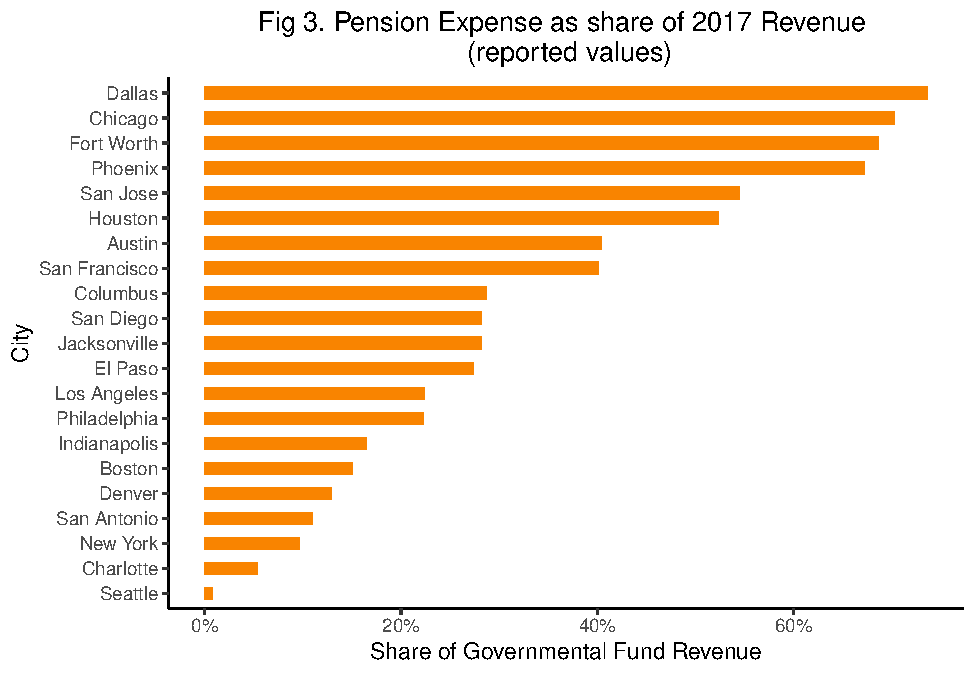
\includegraphics{City-Solvency-Report--Adjusted-_files/figure-latex/unnamed-chunk-8-1.pdf}

\hypertarget{ii.-opeb-liability}{%
\section{II. OPEB Liability}\label{ii.-opeb-liability}}

In this section, we evaluate the other post employment benefit (OPEB)
liability of cities in our study. As before, we report on both a city's
own calculations of their OPEB obligations and how these differ from
valuations using a standardized measure with reasonable discount rate
assumptions. In addition, we provide several ways of comparing the
financial burden due to OPEB.

First, we present the total Unfunded Actuarial Accrued Liability
(UAAL),i.e the difference between the present value of benefit payment
(current and past) and the present value of the OPEB Asset Fund. Second,
we showcase the total UAAL scaled by population size. Finally, we
present the share of city's revenue utilized to cover OPEB benefit
payments.

\hypertarget{unfunded-opeb-liability}{%
\subsubsection{1. Unfunded OPEB
Liability}\label{unfunded-opeb-liability}}

The difference in the reported UAALs and the ones calculated under our
standardized valuation are illustrated in Figure 4 below. As before,
most cities report lower unfunded liabilities than more reasonable
discount rate assumptions would suggest.

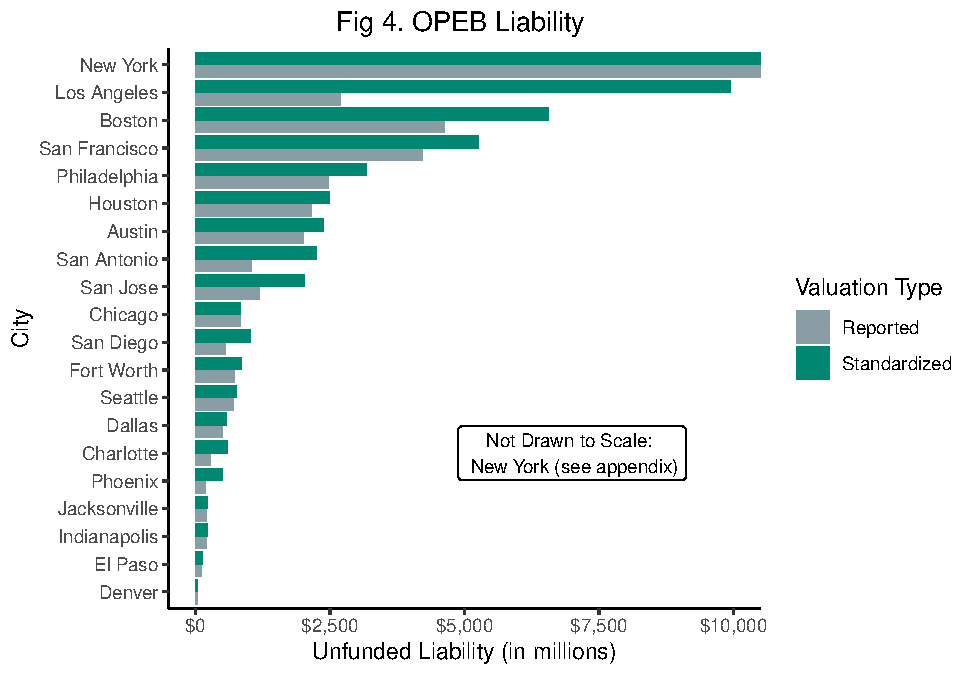
\includegraphics{City-Solvency-Report--Adjusted-_files/figure-latex/unnamed-chunk-9-1.pdf}

Also as expected, cities with the larger populations (New York, Los
Angeles) tend to carry the highest amounts of unfunded obligations,
although there is little correlation between the actual size of city's
obligations and the extent to which they proportionately underestimate
those obligations. While Los Angeles has a dramatic difference between
actual and reported values, so do cities further down the scale, such as
San Antonio, Charlotte, and Phoenix. We also note that there is not
necessarily a clear relation between OPEB obligation and pension
obligation - while Boston, for example, is near the top in regardes to
their OPEB liability, in regards to pensions, they are further down the
list.

\hypertarget{unfunded-opeb-liability-per-capita}{%
\subsubsection{2. Unfunded OPEB Liability Per
Capita}\label{unfunded-opeb-liability-per-capita}}

The difference in the reported UAALs and our own valuations scaled by
population size are illustrated in Figure 5 below. As before, this
allows for an arguably clearer indication of a city's fiscal status.

In addition to allowing for greater comparability between cities in
OPEB, such scale allows for greater comparability with city pension
obligations as well. One thing that obviously arises is how much more
dramatic liability on pensions are than OPEBs. While there are some
liability values near \$10,000, the median per capita OPEB liability is
well under \$5,000, with all but a few cities illustrating obligations
(even by standardized reporting) under \$3,000 per capita and many under
\$1,000. This compares to average standardized obligations of \$14,035
per person per city in the pension arena.

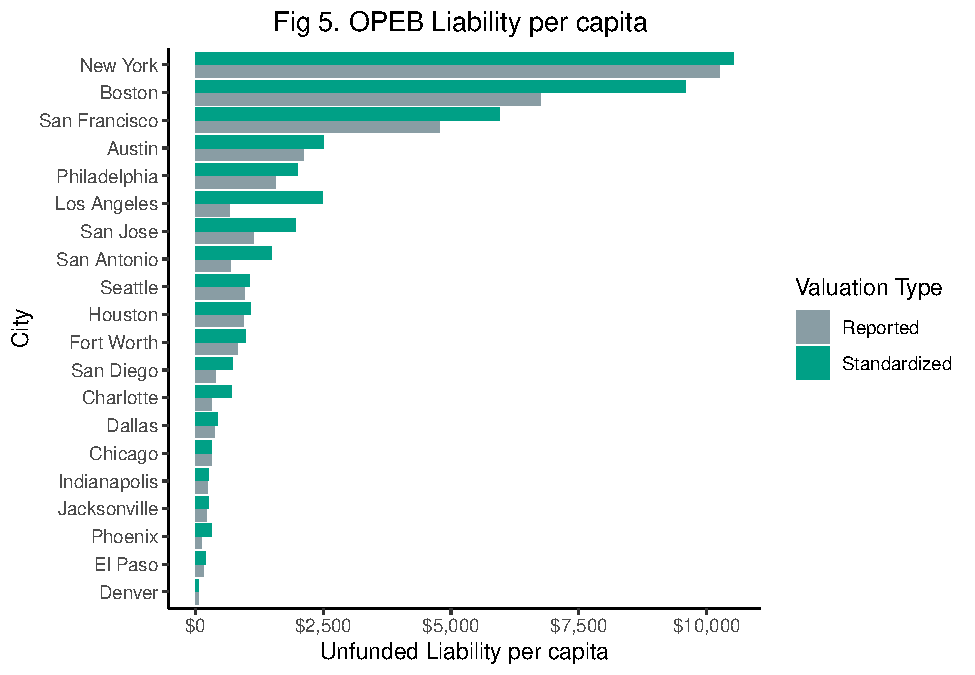
\includegraphics{City-Solvency-Report--Adjusted-_files/figure-latex/unnamed-chunk-10-1.pdf}

\hypertarget{share-of-revenue-1} with
a low of \textbf{0.16\%} for Denver and a high of \textbf{7.2\%} for Los
Angeles. It is interesting to note that the city of New York fares much
better under this metric than the previous ones.

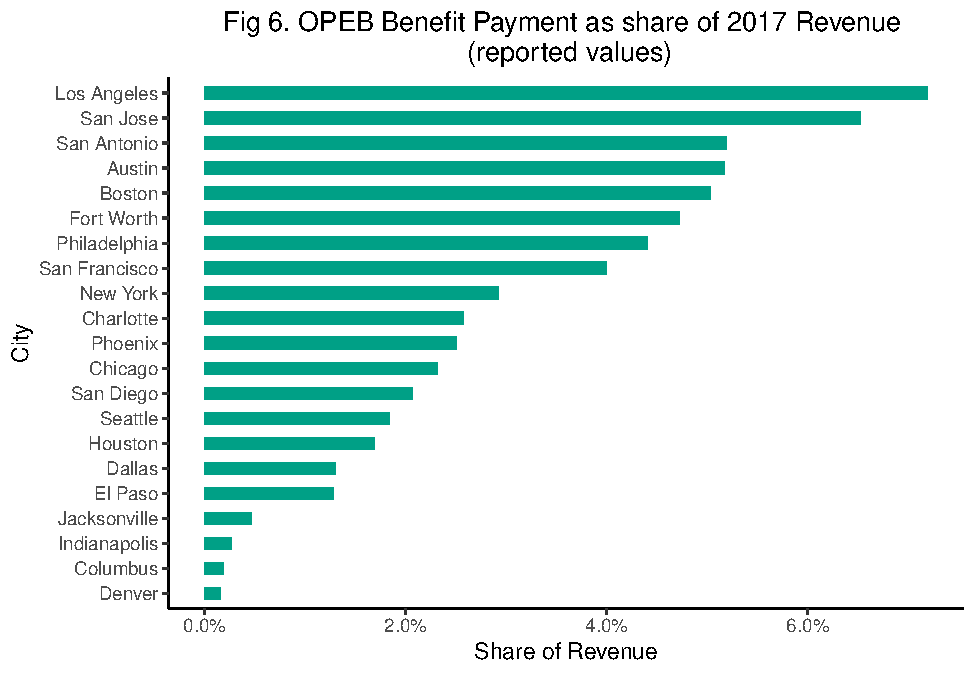
\includegraphics{City-Solvency-Report--Adjusted-_files/figure-latex/unnamed-chunk-11-1.pdf}

\hypertarget{iii.-total-unfunded-liability}{%
\section{III. Total Unfunded
Liability}\label{iii.-total-unfunded-liability}}

In this section, we combine our results from the two previous sections
to study in detail the total unfunded liability of the cities in
question. We report on both their own estimates of their total
obligations as well as a standardized measure. As before, we first
present the total unfunded liability in dollar terms, then showcase the
total liability scaled by population size, and finally display payments
as share of revenue.

\hypertarget{total-unfunded-liability}{%
\subsubsection{1. Total Unfunded
Liability}\label{total-unfunded-liability}}

The difference in the total city reported liabilty (pension and OPEB
combined) and the standardized valuation we calculate are illustrated in
Figure 7 below. Unsurprisingly, for all cities, the standardized total
liability is greater than the reported value. The average reported total
liability was about \textbf{\$27} billion per city while the average
standardized total liability was around \textbf{\$40} billion per city,
with larger cities logically under greater burdens.

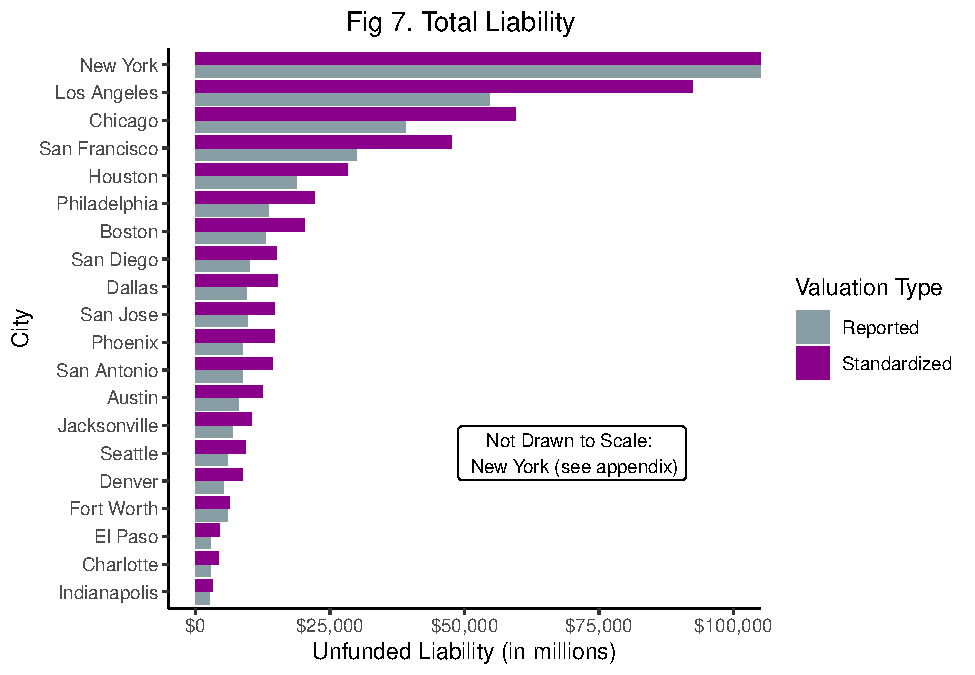
\includegraphics{City-Solvency-Report--Adjusted-_files/figure-latex/unnamed-chunk-12-1.pdf}

\hypertarget{total-unfunded-liability-per-capita}{%
\subsubsection{2. Total Unfunded Liability Per
Capita}\label{total-unfunded-liability-per-capita}}

Figure 8 below shows the total liability per capita for all the cities
included in our report. As before, the total unfunded liabilities these
cities reported were usually lower than our standardized measures, but
the per capita measure allows for a different comparison. In particular,
we note how these numbers are primarily driven by pension numbers, where
obligations tend to be larger.

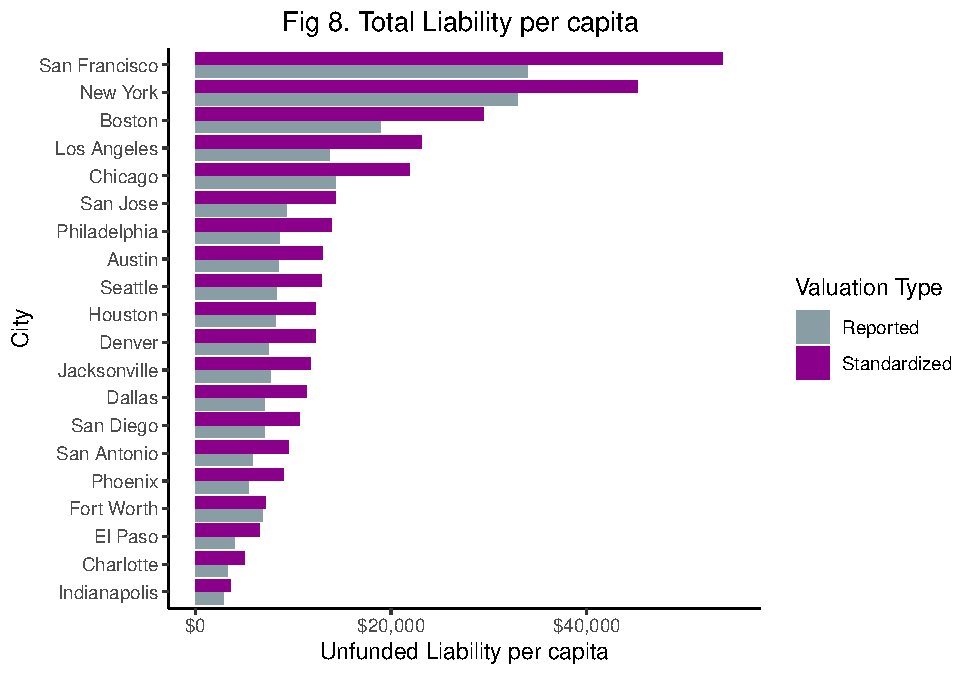
\includegraphics{City-Solvency-Report--Adjusted-_files/figure-latex/unnamed-chunk-13-1.pdf}

\hypertarget{city-pension-and-opeb-payments-and-expenses-as-share-revenue}{%
\subsubsection{3. City Pension and OPEB Payments and Expenses as share
Revenue}\label{city-pension-and-opeb-payments-and-expenses-as-share-revenue}}

Finally, we report overall city pension and OPEB payments and expenses
as a share of revenue, which again illustrates significant diversity
among cities' payments.

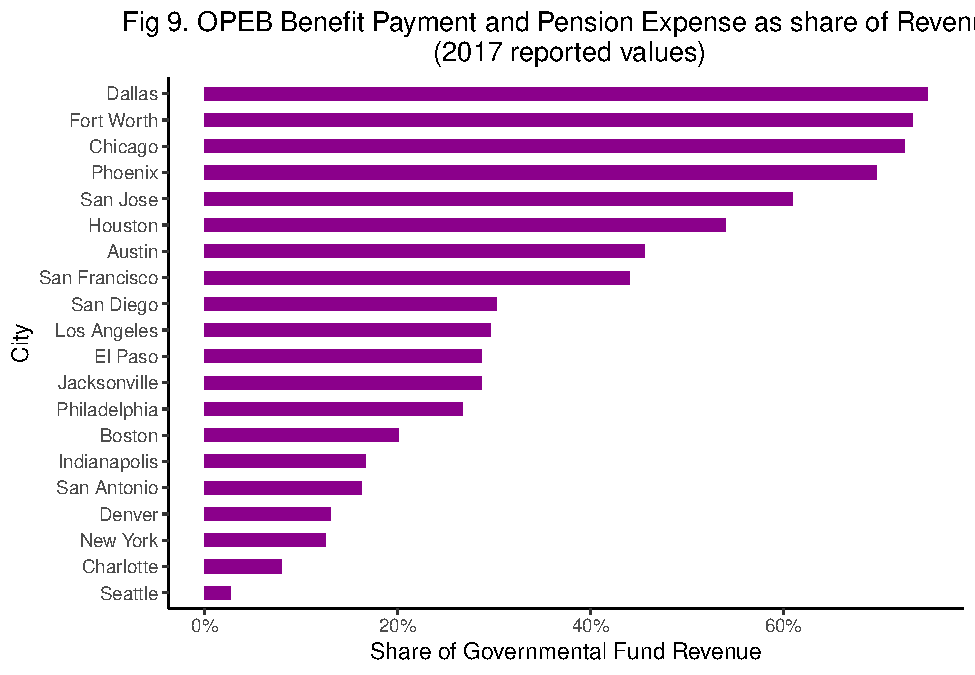
\includegraphics{City-Solvency-Report--Adjusted-_files/figure-latex/unnamed-chunk-14-1.pdf}

\hypertarget{appendix.-discount-rates}{%
\subsubsection{Appendix. Discount
Rates}\label{appendix.-discount-rates}}

The unfunded obligations of local cities with regard to pension and OPEB
plans are sensitive to underlying actuarial assumptions, and even small
changes can significantly change reported liabilities. The most
significant of these assumptions is the discount rate.

In 2004, new reporting guidelines from the Governmental Accounting
Standards Board (GASB) were released. These guidelines, which became
effective in 2007, required cities to report for the cost of both OPEB
and Pension plans on an accrual basis. In particular, GASB Statement
No.~45, Accounting and Financial Reporting by Employers for
Postemployment Benefits Other Than Pensions, represented a significant
change towards accrual reporting for governmental entities.

Although GASB 45 was a major shift in governmental accounting and
financial reporting, it still provides an incentive for governments to
use a higher rate to discount future benefit promises if they set up a
trust and commit to paying the Annual Required Contribution (ARC). The
ARC is the minimum amount required to cover both the plan's normal costs
(the Present Value of benefit payments for the current year) and the
unfunded liability (the gap between current assets and the present value
of future benefits already promised to employees) amortized over a
specific period. Thus, it becomes clear that the discount rate plays a
pivotal role in assessing the ARC. In fact, the higher the discount
rate, the lower the ARC, and vice versa.

In other words, with a trust and a commitment to paying the ARC, cities
can discount obligations by their own estimate of the expected long-term
return of their assets. This idiosyncracy is what makes it problematic
to compare cities according to their own reports: there is wide
variation in discount rates chosen by cities (and sometimes, even by
departments within cities). For example, for OPEB alone, discount rates
for the plans sponsored by the cities in our report ranged from
\textbf{2.92\%} to \textbf{7.95\%} as displayed below in Figure A1.

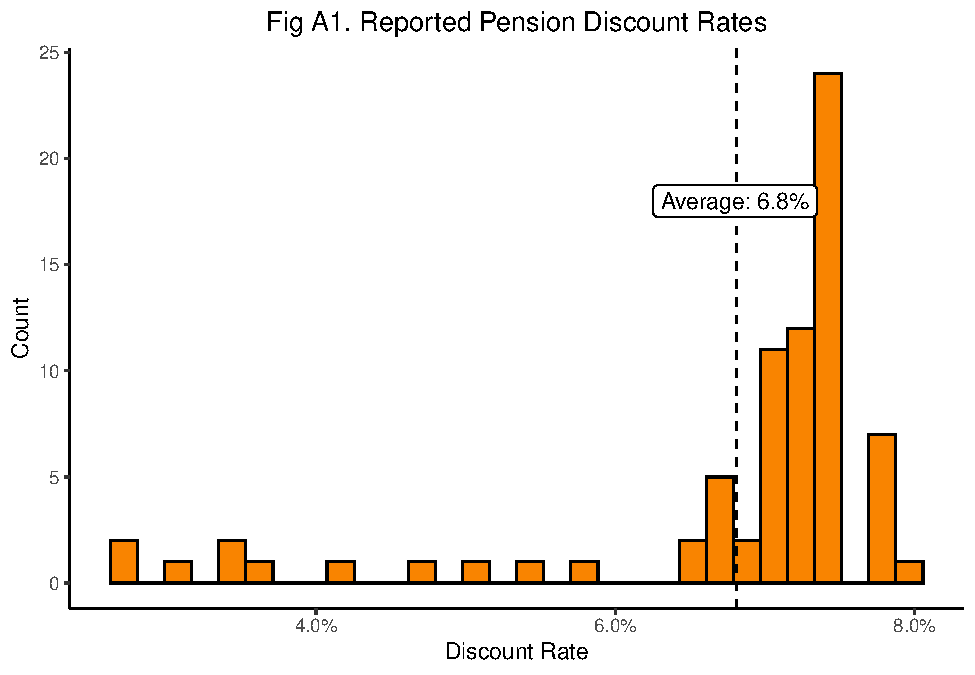
\includegraphics{City-Solvency-Report--Adjusted-_files/figure-latex/unnamed-chunk-15-1.pdf}
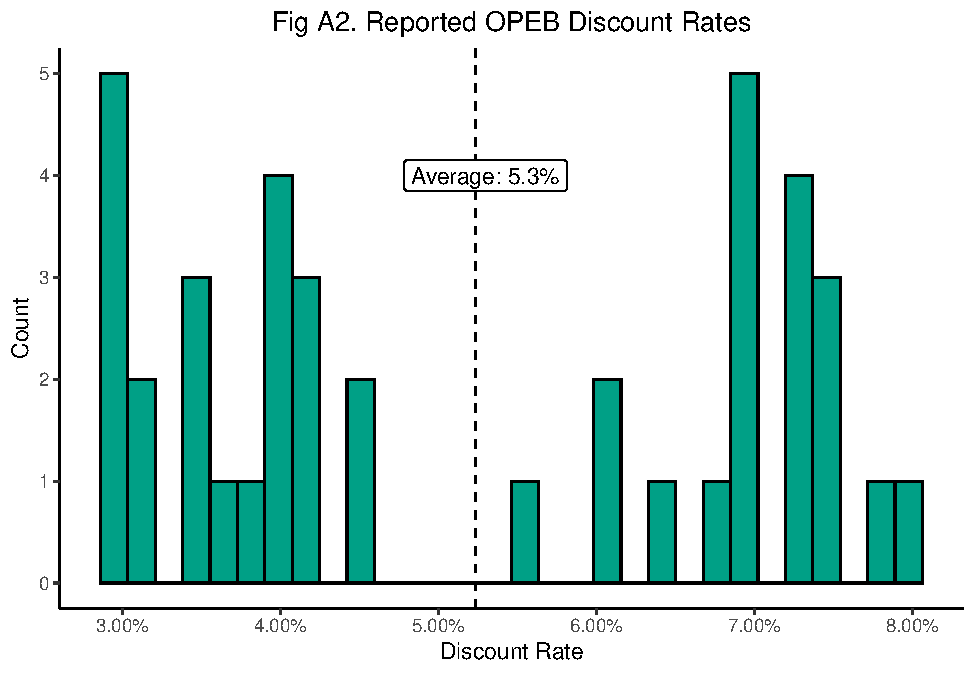
\includegraphics{City-Solvency-Report--Adjusted-_files/figure-latex/unnamed-chunk-15-2.pdf}

\hypertarget{a2.-tables}{%
\subsubsection{A2. Tables}\label{a2.-tables}}

\hypertarget{table-1.-total-pension-and-opeb-liabilities-millions}{%
\paragraph{Table 1. Total Pension and OPEB Liabilities
(Millions)}\label{table-1.-total-pension-and-opeb-liabilities-millions}}

\begin{table}[H]
\centering
\begin{tabular}{l|l|l|l|l}
\hline
City & Pension (Reported) & Pension (Standardized) & OPEB (Reported) & OPEB (Standardized)\\
\hline
Austin & 6,026.22 & 10,004.34 & 2,004.66 & 2,388.49\\
\hline
Boston & 8,336.25 & 13,635.81 & 4,631.37 & 6,569.90\\
\hline
Charlotte & 2,515.18 & 3,683.47 & 276.34 & 601.85\\
\hline
Chicago & 38,113.11 & 58,716.87 & 842.92 & 842.92\\
\hline
Columbus & 5,621.13 & 9,621.40 & NA & NA\\
\hline
Dallas & 8,908.86 & 14,636.43 & 499.91 & 577.88\\
\hline
Denver & 5,250.93 & 8,611.40 & 41.05 & 47.45\\
\hline
El Paso & 2,633.80 & 4,327.22 & 109.74 & 136.32\\
\hline
Fort Worth & 5,318.31 & 5,395.53 & 717.70 & 853.81\\
\hline
Houston & 16,673.85 & 25,807.01 & 2,153.00 & 2,488.78\\
\hline
Indianapolis & 2,330.36 & 2,906.97 & 203.53 & 216.97\\
\hline
Jacksonville & 6,624.00 & 10,273.60 & 198.60 & 229.57\\
\hline
Los Angeles & 51,929.33 & 82,389.56 & 2,701.59 & 9,937.48\\
\hline
Minneapolis & 3,967.82 & 6,518.97 & 34.81 & 37.43\\
\hline
New York & 195,068.92 & 298,844.08 & 88,422.67 & 90,753.81\\
\hline
Philadelphia & 11,168.43 & 18,868.07 & 2,474.54 & 3,172.48\\
\hline
Phoenix & 8,637.08 & 14,190.38 & 185.54 & 510.68\\
\hline
San Antonio & 7,668.03 & 12,003.96 & 1,043.35 & 2,243.07\\
\hline
San Diego & 9,510.89 & 14,068.23 & 553.87 & 1,026.09\\
\hline
San Francisco & 25,777.96 & 42,352.15 & 4,220.04 & 5,261.79\\
\hline
San Jose & 8,456.99 & 12,739.79 & 1,182.08 & 2,029.43\\
\hline
Seattle & 5,303.11 & 8,550.06 & 702.21 & 763.87\\
\hline
\end{tabular}
\end{table}

\hypertarget{table-2.-per-capita-pension-and-opeb-liabilities-thousands}{%
\paragraph{Table 2. Per Capita Pension and OPEB Liabilities
(Thousands)}\label{table-2.-per-capita-pension-and-opeb-liabilities-thousands}}

\begin{table}[H]
\centering
\begin{tabular}{l|l|l|l|l}
\hline
City & Pension (Reported) & Pension (Standardized) & OPEB (Reported) & OPEB (Standardized)\\
\hline
Austin & 6,338.61 & 10,522.97 & 2,108.59 & 2,512.31\\
\hline
Boston & 12,168.04 & 19,903.56 & 6,760.20 & 9,589.79\\
\hline
Charlotte & 2,927.91 & 4,287.92 & 321.69 & 700.61\\
\hline
Chicago & 14,032.81 & 21,618.88 & 310.36 & 310.36\\
\hline
Columbus & 6,393.68 & 10,943.73 & NA & NA\\
\hline
Dallas & 6,643.45 & 10,914.56 & 372.79 & 430.93\\
\hline
Denver & 7,442.93 & 12,206.24 & 58.18 & 67.25\\
\hline
El Paso & 3,852.96 & 6,330.26 & 160.54 & 199.42\\
\hline
Fort Worth & 6,083.85 & 6,172.19 & 821.01 & 976.71\\
\hline
Houston & 7,208.75 & 11,157.37 & 930.83 & 1,075.99\\
\hline
Indianapolis & 2,670.35 & 3,331.09 & 233.23 & 248.63\\
\hline
Jacksonville & 7,425.49 & 11,516.69 & 222.63 & 257.35\\
\hline
Los Angeles & 12,982.33 & 20,597.39 & 675.40 & 2,484.37\\
\hline
Minneapolis & 9,395.05 & 15,435.69 & 82.42 & 88.63\\
\hline
New York & 22,621.93 & 34,656.63 & 10,254.28 & 10,524.62\\
\hline
Philadelphia & 7,064.15 & 11,934.26 & 1,565.17 & 2,006.63\\
\hline
Phoenix & 5,311.86 & 8,727.17 & 114.11 & 314.07\\
\hline
San Antonio & 5,112.02 & 8,002.64 & 695.57 & 1,495.38\\
\hline
San Diego & 6,697.81 & 9,907.20 & 390.05 & 722.60\\
\hline
San Francisco & 29,148.62 & 47,890.01 & 4,771.84 & 5,949.81\\
\hline
San Jose & 8,171.00 & 12,308.97 & 1,142.11 & 1,960.80\\
\hline
Seattle & 7,317.20 & 11,797.33 & 968.90 & 1,053.99\\
\hline
\end{tabular}
\end{table}

\end{document}
